\documentclass{standalone}
\usepackage{tikz}
\usetikzlibrary{patterns, positioning}
\usepackage[sfdefault]{ClearSans} %% option 'sfdefault' activates Clear Sans as the default text font
\usepackage[T1]{fontenc}

\begin{document}
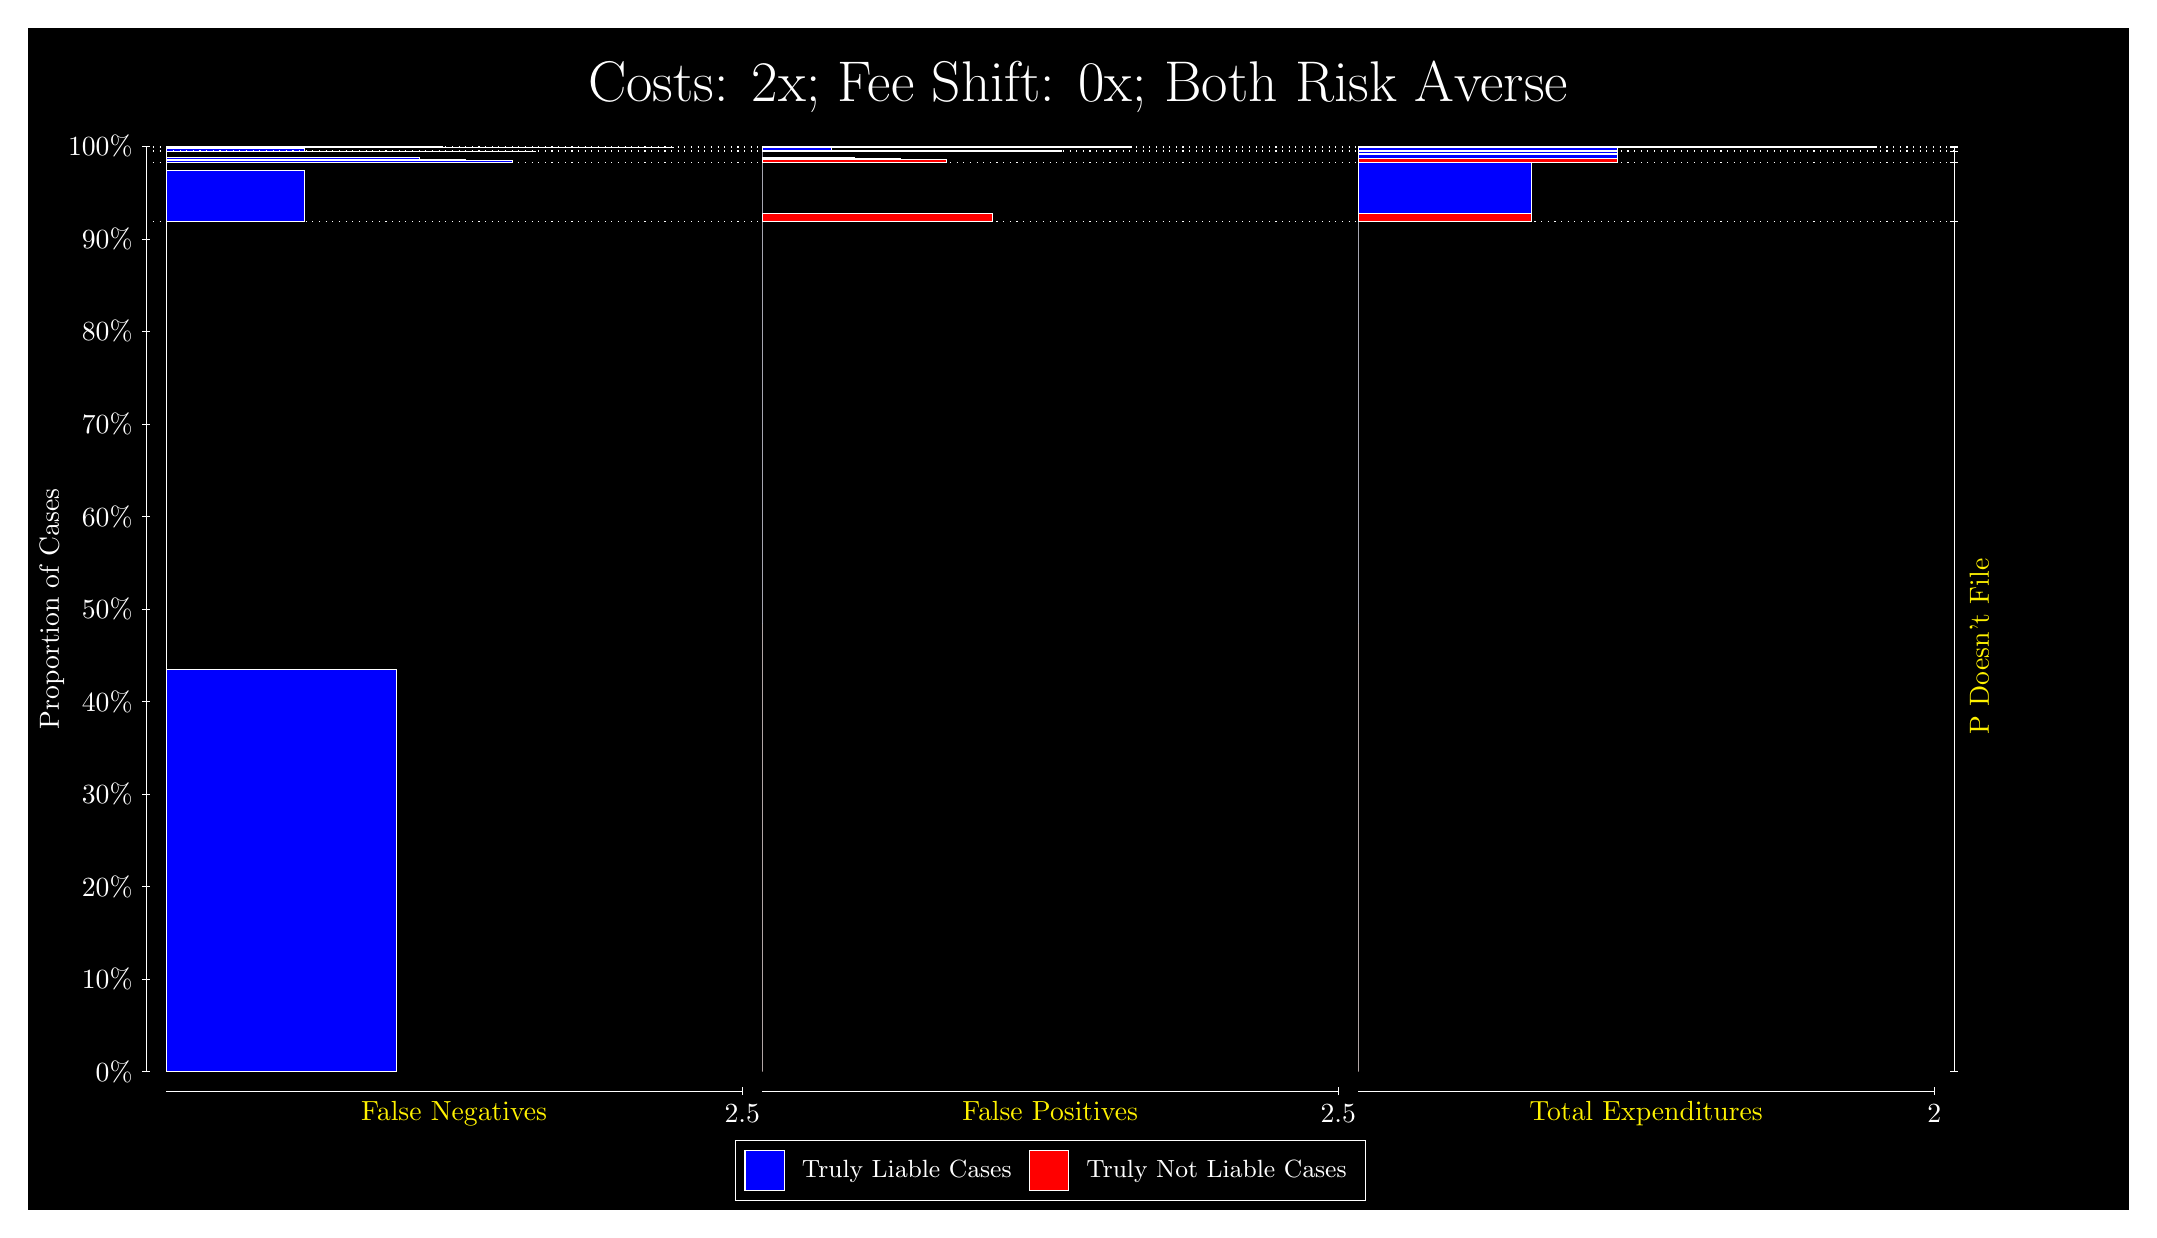
\begin{tikzpicture}
\draw[fill=black] (0,0) rectangle (26.667,15);
\draw[text=white] (0,13.5) rectangle (26.667,15) node[midway] {\huge Costs: 2x; Fee Shift: 0x; Both Risk Averse};
\draw[white, very thin] (1.5,1.75) -- (1.5,13.5);
\node[rotate=90, text=white, anchor=center] at (0.3, 7.625) {Proportion of Cases};
\draw[white, very thin] (1.45,1.75) -- (1.55,1.75);
\node[text=white, anchor=east] at (1.45, 1.75) {0\%};
\draw[white, very thin] (1.45,2.925) -- (1.55,2.925);
\node[text=white, anchor=east] at (1.45, 2.925) {10\%};
\draw[white, very thin] (1.45,4.1) -- (1.55,4.1);
\node[text=white, anchor=east] at (1.45, 4.1) {20\%};
\draw[white, very thin] (1.45,5.275) -- (1.55,5.275);
\node[text=white, anchor=east] at (1.45, 5.275) {30\%};
\draw[white, very thin] (1.45,6.45) -- (1.55,6.45);
\node[text=white, anchor=east] at (1.45, 6.45) {40\%};
\draw[white, very thin] (1.45,7.625) -- (1.55,7.625);
\node[text=white, anchor=east] at (1.45, 7.625) {50\%};
\draw[white, very thin] (1.45,8.8) -- (1.55,8.8);
\node[text=white, anchor=east] at (1.45, 8.8) {60\%};
\draw[white, very thin] (1.45,9.975) -- (1.55,9.975);
\node[text=white, anchor=east] at (1.45, 9.975) {70\%};
\draw[white, very thin] (1.45,11.15) -- (1.55,11.15);
\node[text=white, anchor=east] at (1.45, 11.15) {80\%};
\draw[white, very thin] (1.45,12.325) -- (1.55,12.325);
\node[text=white, anchor=east] at (1.45, 12.325) {90\%};
\draw[white, very thin] (1.45,13.5) -- (1.55,13.5);
\node[text=white, anchor=east] at (1.45, 13.5) {100\%};

\draw[white, very thin] (24.457,1.75) -- (24.457,13.5);
\draw[white, very thin] (24.407,1.75) -- (24.507,1.75);
\node[anchor=west] at (24.407, 1.75) {};
\draw[white, very thin] (24.407,12.548) -- (24.507,12.548);
\node[anchor=west] at (24.407, 12.548) {};
\draw[white, very thin] (24.407,13.295) -- (24.507,13.295);
\node[anchor=west] at (24.407, 13.295) {};
\draw[white, very thin] (24.407,13.431) -- (24.507,13.431);
\node[anchor=west] at (24.407, 13.431) {};
\draw[white, very thin] (24.407,13.443) -- (24.507,13.443);
\node[anchor=west] at (24.407, 13.443) {};
\draw[white, very thin] (24.407,13.488) -- (24.507,13.488);
\node[anchor=west] at (24.407, 13.488) {};
\draw[white, very thin] (24.407,13.493) -- (24.507,13.493);
\node[anchor=west] at (24.407, 13.493) {};
\draw[white, very thin] (24.407,13.5) -- (24.507,13.5);
\node[anchor=west] at (24.407, 13.5) {};

\draw[white, very thin, fill=blue] (1.75,1.75) rectangle (4.6775,6.8609);
\draw[white, very thin, fill=red] (1.75,6.8609) rectangle (1.75,12.548);
\draw[white, very thin, fill=blue] (1.75,12.548) rectangle (3.5065,13.197);
\draw[white, very thin, fill=red] (1.75,13.197) rectangle (1.75,13.295);
\draw[white, very thin, fill=blue] (1.75,13.295) rectangle (6.1413,13.317);
\draw[white, very thin, fill=blue] (1.75,13.317) rectangle (5.5558,13.332);
\draw[white, very thin, fill=blue] (1.75,13.332) rectangle (4.9703,13.361);
\draw[white, very thin, fill=red] (1.75,13.361) rectangle (1.75,13.431);
\draw[white, very thin, fill=blue] (1.75,13.431) rectangle (6.4341,13.437);
\draw[white, very thin, fill=red] (1.75,13.437) rectangle (1.75,13.443);
\draw[white, very thin, fill=blue] (1.75,13.443) rectangle (3.5065,13.478);
\draw[white, very thin, fill=red] (1.75,13.478) rectangle (1.75,13.488);
\draw[white, very thin, fill=blue] (1.75,13.488) rectangle (8.1906,13.49);
\draw[white, very thin, fill=red] (1.75,13.49) rectangle (1.75,13.493);
\draw[white, very thin, fill=blue] (1.75,13.493) rectangle (5.2631,13.498);
\draw[white, very thin, fill=red] (1.75,13.498) rectangle (1.75,13.5);
\draw[white, very thin, fill=red] (9.3189,1.75) rectangle (9.3189,7.4367);
\draw[white, very thin, fill=blue] (9.3189,7.4367) rectangle (9.3189,12.548);
\draw[white, very thin, fill=red] (9.3189,12.548) rectangle (12.246,12.645);
\draw[white, very thin, fill=blue] (9.3189,12.645) rectangle (9.3189,13.295);
\draw[white, very thin, fill=red] (9.3189,13.295) rectangle (11.661,13.333);
\draw[white, very thin, fill=red] (9.3189,13.333) rectangle (11.075,13.347);
\draw[white, very thin, fill=red] (9.3189,13.347) rectangle (10.49,13.365);
\draw[white, very thin, fill=blue] (9.3189,13.365) rectangle (9.3189,13.431);
\draw[white, very thin, fill=red] (9.3189,13.431) rectangle (10.197,13.437);
\draw[white, very thin, fill=blue] (9.3189,13.437) rectangle (9.3189,13.443);
\draw[white, very thin, fill=red] (9.3189,13.443) rectangle (13.125,13.453);
\draw[white, very thin, fill=blue] (9.3189,13.453) rectangle (10.197,13.488);
\draw[white, very thin, fill=red] (9.3189,13.488) rectangle (11.075,13.491);
\draw[white, very thin, fill=blue] (9.3189,13.491) rectangle (9.3189,13.493);
\draw[white, very thin, fill=red] (9.3189,13.493) rectangle (14.003,13.495);
\draw[white, very thin, fill=blue] (9.3189,13.495) rectangle (11.075,13.5);
\draw[white, very thin, fill=red] (16.888,1.75) rectangle (16.888,7.4367);
\draw[white, very thin, fill=blue] (16.888,7.4367) rectangle (16.888,12.548);
\draw[white, very thin, fill=red] (16.888,12.548) rectangle (19.083,12.645);
\draw[white, very thin, fill=blue] (16.888,12.645) rectangle (19.083,13.295);
\draw[white, very thin, fill=red] (16.888,13.295) rectangle (20.181,13.351);
\draw[white, very thin, fill=blue] (16.888,13.351) rectangle (20.181,13.402);
\draw[white, very thin, fill=red] (16.888,13.402) rectangle (20.181,13.416);
\draw[white, very thin, fill=blue] (16.888,13.416) rectangle (20.181,13.431);
\draw[white, very thin, fill=red] (16.888,13.431) rectangle (20.181,13.437);
\draw[white, very thin, fill=blue] (16.888,13.437) rectangle (20.181,13.443);
\draw[white, very thin, fill=red] (16.888,13.443) rectangle (20.181,13.453);
\draw[white, very thin, fill=blue] (16.888,13.453) rectangle (20.181,13.488);
\draw[white, very thin, fill=red] (16.888,13.488) rectangle (23.475,13.491);
\draw[white, very thin, fill=blue] (16.888,13.491) rectangle (23.475,13.493);
\draw[white, very thin, fill=red] (16.888,13.493) rectangle (23.475,13.495);
\draw[white, very thin, fill=blue] (16.888,13.495) rectangle (23.475,13.5);
\draw[white, dotted] (1.5,12.548) -- (24.457,12.548);
\draw[white, dotted] (1.5,13.295) -- (24.457,13.295);
\draw[white, dotted] (1.5,13.431) -- (24.457,13.431);
\draw[white, dotted] (1.5,13.443) -- (24.457,13.443);
\draw[white, dotted] (1.5,13.488) -- (24.457,13.488);
\draw[white, dotted] (1.5,13.493) -- (24.457,13.493);
\draw[white, very thin] (1.75,1.5) -- (9.0689,1.5);
\node[text=yellow, anchor=north] at (5.4094, 1.5) {False Negatives};
\draw[white, very thin] (9.0689,1.45) -- (9.0689,1.55);
\node[text=white, anchor=north] at (9.0689, 1.45) {2.5};

\draw[white, very thin] (9.3189,1.5) -- (16.638,1.5);
\node[text=yellow, anchor=north] at (12.978, 1.5) {False Positives};
\draw[white, very thin] (16.638,1.45) -- (16.638,1.55);
\node[text=white, anchor=north] at (16.638, 1.45) {2.5};

\draw[white, very thin] (16.888,1.5) -- (24.207,1.5);
\node[text=yellow, anchor=north] at (20.547, 1.5) {Total Expenditures};
\draw[white, very thin] (24.207,1.45) -- (24.207,1.55);
\node[text=white, anchor=north] at (24.207, 1.45) {2};

\node[text=yellow, centered, rotate=90] at (24.777, 7.1488) {P Doesn't File};







\draw (12.978300999999998,1.5) node[draw=none] (baseCoordinate) {};
\begin{scope}[align=center]
        \matrix[scale=0.5, draw=white, below=0.5cm of baseCoordinate, nodes={draw}, column sep=0.1cm]{
            \node[rectangle, draw, minimum width=0.5cm, minimum height=0.5cm, fill=blue] {}; &
            \node[draw=none, font=\small, text=white] (B) {Truly Liable Cases}; &
            \node[rectangle, draw, minimum width=0.5cm, minimum height=0.5cm, fill=red] {}; &
            \node[draw=none, font=\small, text=white] (B) {Truly Not Liable Cases}; \\
            };
\end{scope}

\end{tikzpicture}
\end{document}